\subsection{Beispiel: knn-Klassifikation}\label{maschinelleslernen:knnklassifikation}
Der knn-Algorithmus ist einer der bekanntesten Algorithmus aus dem Bereich Klassifikation und wird daher hier als Codebeispiel dargestellt und erl�utert.

Folgende Imports\randnotiz{Imports} sind f�r dieses Beispiel n�tig:
\lstinputlisting[language=Python,firstline=4,lastline=11]{chapters/advancedTopics/src/machinelearning/knnsample.py}\label{knnsample:lst:knnsample4}

Anschlie�end k�nnen die Daten\randnotiz{Daten laden} geladen und die Spaltennamen definiert werden.
\lstinputlisting[language=Python,firstline=14,lastline=20]{chapters/advancedTopics/src/machinelearning/knnsample.py}\label{knnsample:lst:knnsample14}

Jetzt werden die Daten gelesen\randnotiz{Daten lesen und vorbereiten} und vorbereitet.
\lstinputlisting[language=Python,firstline=22,lastline=28]{chapters/advancedTopics/src/machinelearning/knnsample.py}\label{knnsample:lst:knnsample22}

Zur Berechnung m�ssen die Daten\randnotiz{Daten skalieren} skaliert werden.
\lstinputlisting[language=Python,firstline=33,lastline=37]{chapters/advancedTopics/src/machinelearning/knnsample.py}\label{knnsample:lst:knnsample33}

Nun kann der KNN-Algorithmus\randnotiz{Algorithmus anwenden} angewendet werden.
\lstinputlisting[language=Python,firstline=39,lastline=44]{chapters/advancedTopics/src/machinelearning/knnsample.py}\label{knnsample:lst:knnsample39}

Jetzt k�nnen wir die Daten-Matrix\randnotiz{Matrix ausgeben} ausgeben.
\lstinputlisting[language=Python,firstline=46,lastline=47]{chapters/advancedTopics/src/machinelearning/knnsample.py}\label{knnsample:lst:knnsample46}

Als Ausgabe wird Folgendes angezeigt
\begin{lstlisting}
[[ 9  0  0]
 [ 0 12  1]
 [ 0  1  7]]
\end{lstlisting} 
 
Zus�tzlich\randnotiz{Report ausgeben} kann ein Report angezeigt werden, welcher eine gute �bersicht �ber die klassifizierten Daten gibt.
\lstinputlisting[language=Python,firstline=48,lastline=49]{chapters/advancedTopics/src/machinelearning/knnsample.py}\label{knnsample:lst:knnsample49}

Die Ausgabe ist die folgende:
\begin{lstlisting} 
                  precision    recall  f1-score   support
 
     Iris-setosa       1.00      1.00      1.00         9
 Iris-versicolor       0.92      0.92      0.92        13
  Iris-virginica       0.88      0.88      0.88         8
 
       micro avg       0.93      0.93      0.93        30
       macro avg       0.93      0.93      0.93        30
    weighted avg       0.93      0.93      0.93        30
\end{lstlisting}



Um \randnotiz{Fehler ausgeben}ein abschlie�endes Bild �ber die Klassifikation zu erhalten k�nnen nun noch die Fehler ausgegeben werden.
\lstinputlisting[language=Python,firstline=51,lastline=61]{chapters/advancedTopics/src/machinelearning/knnsample.py}\label{knnsample:lst:knnsample51}


Aus\randnotiz{Fehler-Plot erzeugen} den berechneten Fehlern bei der Klassifikation kann nun noch ein Plot erzeugt werden.
\lstinputlisting[language=Python,firstline=64,lastline=72]{chapters/advancedTopics/src/machinelearning/knnsample.py}\label{knnsample:lst:knnsample64}

Der Plot zeigt sich wie in Abbildung ~\ref{ml:samples:plotknn}.

\begin{figure}[ht]
	\centering
	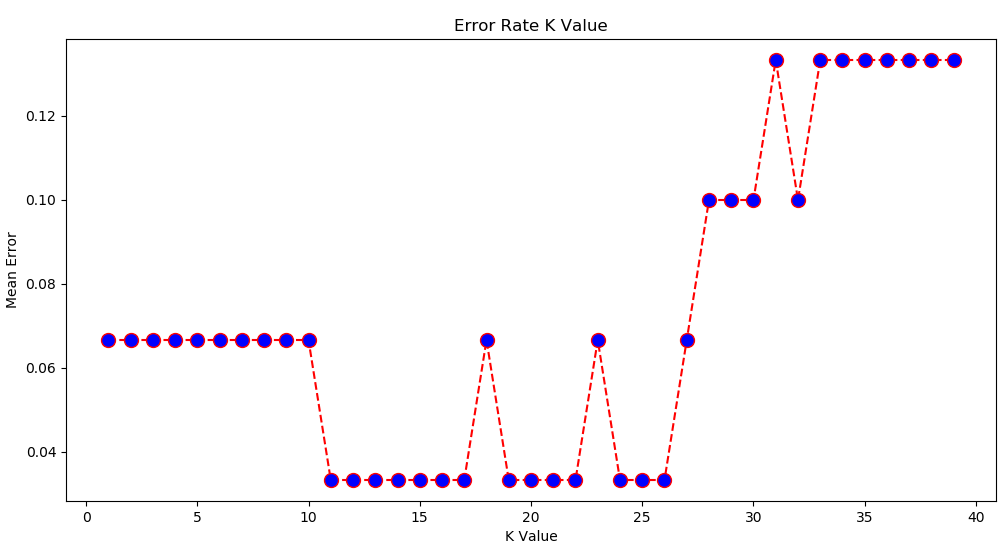
\includegraphics[width=1\textwidth]{images/MachineLearning/ml_knn_plot.png}
	\caption{Ergebnis-Plot der Fehler nach Ausf�hrung KNN}
	\label{ml:samples:plotknn}
\end{figure}

\uebung
\aufgabe{MachineLearning/machinelearning_knn}
